\section{Motivation}
\begin{figure}
  \begin{centering}
      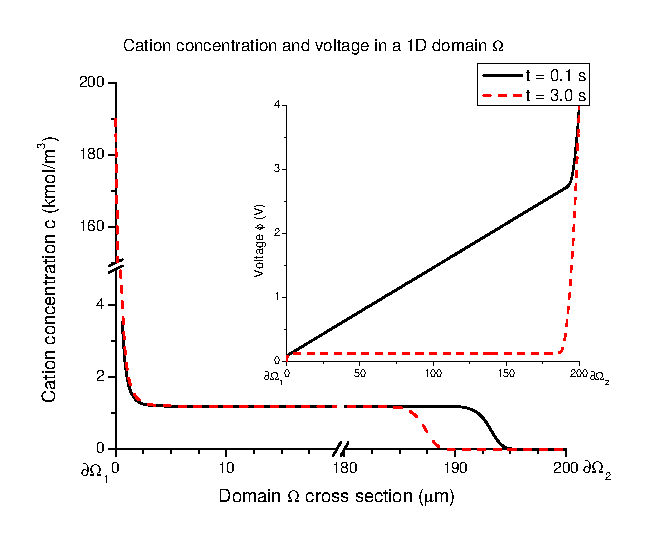
\includegraphics[]{comsol_conc_volt}
  \caption{\label{fig:comsol-conc-volt}Calculated concentration $C$ and voltage $\phi$
  in a 1D domain $\Omega\subset\mathbb{R}$.
  Dirichlet boundary conditions ($V_{\partial \Omega_1}=0\ V$
  and $V_{\partial \Omega_2}=4\ V$) were
	applied to the Poisson equation Eq.~\eqref{eq:poisson} and Neumann boundaries
	to the Nernst-Planck equation Eq.~\eqref{eq:nernst-planck}.}
  \end{centering}
\end{figure}
Fig.~\ref{fig:comsol-conc-volt} shows a solution for $C$ and $\phi$ in
the time dependent NPN system at $t=0.1\ s$ and $t=3.0\ s$. Solution
constants are shown in Table~\ref{Table:used-constants}.
It can be seen that the solution has two notable characteristics. 
Firstly, $\nabla C$ at $\partial \Omega_2$ is
moving in time, whereas $\nabla C$ at $\partial \Omega_1$ is very
sharp. For the large part of the domain $\Omega$ $\nabla C=0$.
At the same time, $\phi$ is a rather smooth fucntion in $\Omega$.
This clearly makes the choice of mesh for the time dependent NPN
system difficult. By creating a too fine mesh, the problem gets
too big. By choosing a coarser mesh, the calculation error goes up.
Furthermore, from the shape of the solution in Fig.~\ref{fig:comsol-conc-volt}
can be seen that the polynomial degree of the elements in the middle
of the domain $\Omega$ and near the boundaries $\partial \Omega_1,\ \partial \Omega_2$
should be different --- namely higher degree near the boundaries. 
Overall shape of the solutions suggest that
using different meshes for variables $C$ and $\phi$ can be beneficial
in terms of resources and calculation time.

All the aforementioned difficulties can be solved by using
a time dependent adaptive multimesh \emph{hp}-FEM solver.
Automatic time dependent adaptivity in conjuction with \emph{hp}-FEM 
helps to limit the error of the calculations by choosing
a suitable mesh and polynomial degrees of the elements at each time step.
In this work Hermes2D~\cite{Hermes-project} was used to study
the problem size, error convergence and solution time of NPN system 
with different adaptivity algorithms.

\begin{table}
\caption{Constants used in the Poisson-Nernst-Planck system of equations.}
\centering
\label{Table:used-constants}
{
\begin{tabular}{llll}
  \hline \hline
  Constant&Value&Unit&Description\\
  \hline
  $D$&$10\times10^{-11}$&$\frac{m^2}{s}$&Diffusion constant\\
  $z$&1&-&Charge number\\
  $F$&96,485&$\frac{C}{mol}$&Faraday number\\
  $R$&8.31&$\frac{J}{mol\cdot K}$&The gas constant\\
  $\mu\ \left( = \frac{D}{RT}\right)$&$4.11\times 10^{-14}$&$\frac{s}{mol\cdot K}$&Mobility\\
  $C_{0}$&1,200&$\frac{mol}{m^3}$&Anion concentration\\
  $\varepsilon$&0.025&$\frac{F}{m}$&Electric permittivity\\
  \hline
  \hline
\end{tabular}
}
\end{table}

\subsection{Practical application}
IPMCs have been studied in past two decades in view of using them
as noiseless mechanoelectrical or electromechanical transducers.
The advantages of the IPMCs over other electroactive polymer actuators
are low voltage bending, high strains ($>1\%$), and ability to work
in wet environments. A typical IPMC consists of a thin sheet of polymer
(often Nafion or Teflon) which is sandwiched between noble
metal electrodes such as platinum or gold. When fabricated, the polymer 
membrane is saturated with certain solvent and ions, e.g water and $H^+$.
When a voltage is applied to the eletrodes, the counter ions start
migrating due to the imposed electric field. By dragging along the solvent,
the osmotic pressure difference near the electrodes occur which in turn
results in bending of the material (see Fig.~\ref{fig:conceptual}).
\begin{figure}
  \begin{centering}
    \subfloat[~]{\begin{centering}
      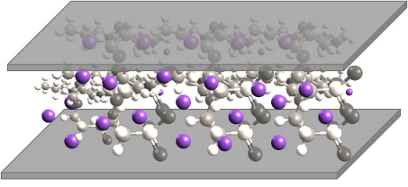
\includegraphics[scale=0.6]{IPMC}
      \par\end{centering}}~
    \subfloat[~]{\begin{centering}
      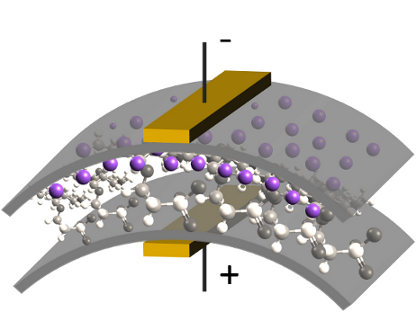
\includegraphics[scale=0.6]{IPMC_bent}
      \par\end{centering}}
  \par\end{centering}
  \caption{\label{fig:conceptual}Conceptual model of the actuation
 	of IPMC. Initial counter ion distribution (a) and
	the distribution and resulting bending after applying a voltage (b).}
\end{figure}
The derived and implemented model helps to predict the actuation of the
material. Furthermore, it is expected that the \emph{hp}-FEM implementation
results in a smaller problem size, thus likely allowing faster calculation
in both 2D and 3D.



